\section{Sentence generation as planning}
\label{sec:crisp}


We consider a planning domain that comes up in the generation of
natural language sentences based on tree-adjoining grammar (TAG;
\cite{joshi;etal1997}).  This is a standard problem in computational
linguistics, which we sketch by example; see
\cite{Stone2003a,KolSto07} for details.

% \begin{figure}
%   \centering
%   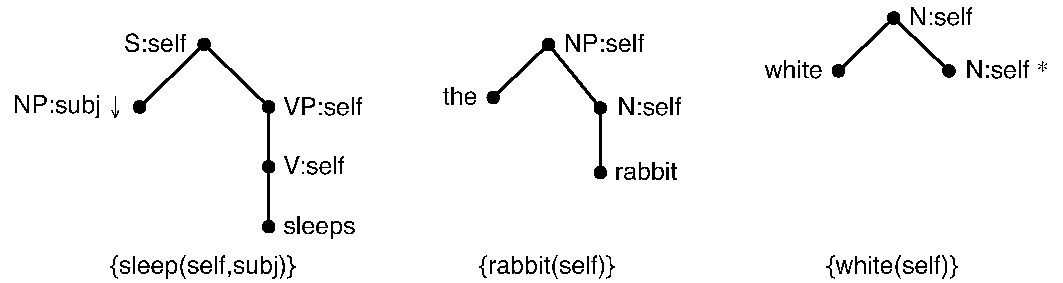
\includegraphics[width=0.75\columnwidth]{pic-grammar}
%   \caption{An example grammar in the sentence generation domain.}
%   \label{fig:white-rabbit-sleeps-grammar}
% \end{figure}

\begin{figure}
  \centering
  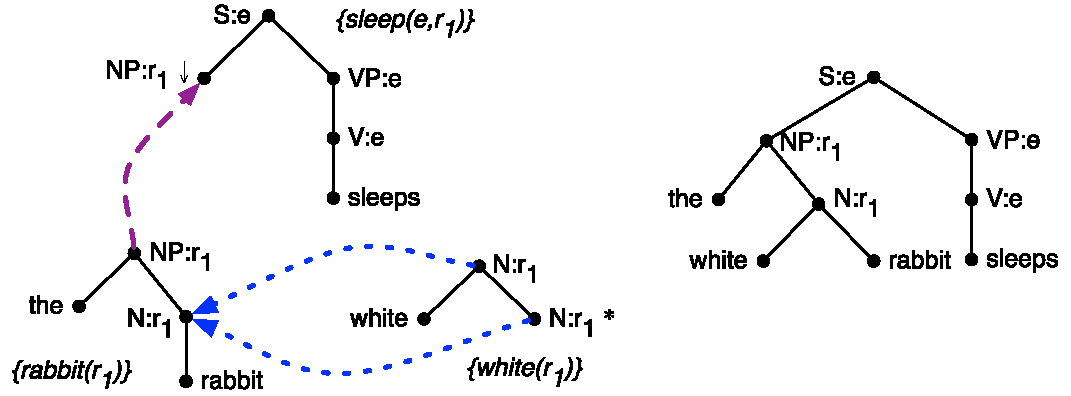
\includegraphics[width=1\columnwidth]{pic-derivation}
  \caption{Derivation of ``The white rabbit sleeps.''}
  \label{fig:white-rabbit-sleeps-deriv}
\end{figure}

A TAG grammar consists of a finite set of \emph{elementary trees},
each of which contains one or more words; the left of
Fig.~\ref{fig:white-rabbit-sleeps-deriv} shows three trees for ``the
rabbit'', ``sleeps'', and ``white''.  Trees can be combined using the
operations of \emph{substitution} (purple dashed arrow in the figure)
and \emph{adjunction} (blue dotted arrows) to form larger trees.
The end result of a grammatically correct derivation is a tree all of
whose leaves are labeled with words, as on the right of
Fig.~\ref{fig:white-rabbit-sleeps-deriv}. We can read off a sentence
from such a tree from left to right.

To use TAG grammars for generation \cite{Stone2003a}, we assume a set
of ground atoms expressing the information we want the sentence to
convey, such as $\{\mathsf{sleep}(e,r_1)\}$, and a knowledge base that
contains all ground atoms we know to be true; say,
$\{\mathsf{sleep}(e,r_1), \mathsf{rabbit}(r_1), \mathsf{rabbit}(r_2),
\mathsf{white}(r_1), \mathsf{brown}(r_2)\}$.  We then add variables
ranging over constants from the knowledge base to the nodes of each
elementary tree, and equip every elementary tree with a set of atoms
over these variables to encode the meaning this tree expresses
(printed in italics in the figure).
Fig.~\ref{fig:white-rabbit-sleeps-deriv} already shows specific
instances of the elementary trees from the grammar, in which constants
have been substituted for these variables.  The derivation in the
figure conveys the intended meaning -- in particular, that $r_1$
sleeps.  Crucially, it also describes uniquely who does the sleeping:
The sentence ``the rabbit sleeps'' would not have done this, as ``the
rabbit'' could be understood either as $r_1$ or $r_2$.  We say that
$r_2$ is a \emph{distractor} for the subject of the sentence, which is
removed by adjoining the tree for ``white''.  In short, the sentence
generation problem consists in computing a grammatically correct TAG
derivation from instances of the elementary trees in the grammar that
conveys the intended meaning and describes all referents uniquely.




\subsection{Sentence generation as a planning problem}

The TAG sentence generation problem can be encoded as a planning
problem \cite{KolSto07}.  The key idea is that each operator encodes
the addition of an elementary tree to the derivation; the syntactic
and semantic requirements and effects of doing this are captured in
the operator's precondition and effect.


\newcommand{\action}[4]{\textbf{#1$(#2)$:}\\
\strut\quad   Precond:$\;$ \parbox[t]{12cm}{\ensuremath{#3}}\\
\strut\quad   Effect:$\;$ \parbox[t]{12cm}{\ensuremath{#4}}}
\newcommand{\f}[1]{\mathsf{#1}}

\begin{figure}
%\centering
%\begin{minipage}{0.8\textwidth}
{\small%
\action{sleeps}{u, u_1, u_n, x_0, x_1}{
  \f{subst}(\f{S},u) \wedge \f{ref}(u,x_0) \wedge
  \f{sleep}(x_0,x_1) \\ \wedge \f{current}(u_1) \wedge
  \f{next}(u_1,u_n)
}{
  \neg \f{subst}(\f{S},u) \wedge \f{expressed}(\f{sleep}, x_0, x_1) \\
  \wedge \f{subst}(\f{NP},u) \wedge \f{ref}(u_1,x_1) \\ \wedge
  \neg \f{current}(u_1) \wedge \f{current}(u_n) \\ \wedge
  \forall y. y \neq x_1 \rightarrow \f{distractor}(u_1,y)
}\\

\action{rabbit}{u, x_0}{
  \f{subst}(\f{NP},u) \wedge \f{ref}(u,x_0) \wedge \f{rabbit}(x_0)
}{
  \neg \f{subst}(\f{NP},u) \wedge \f{canadjoin}(\f{N},u) \\
  \wedge \forall y. \neg \f{rabbit}(y) \rightarrow \neg \f{distractor}(u,y)
}\\

\action{white}{u,x_0}{
  \f{canadjoin}(\f{N},u) \wedge \f{ref}(u,x_0) \wedge \f{rabbit}(x_0)
}{
  \forall y. \neg \f{white}(y) \rightarrow \neg \f{distractor}(u,y)
}
}\strut\\[-5ex]
%\end{minipage}
\caption{Actions for generating ``The white rabbit
sleeps.''}
\label{fig:white-rabbit-as-planning}
\end{figure}

More precisely, each operator has a parameter $u$ representing the
syntax node into which the elementary tree is substituted or adjoined,
and a parameter $u_i$ for each substitution node.  There are also
parameters $x_0,\ldots,x_k$ for the variables in the semantic
representation of the elementary tree; $x_0$ is the variable that
occurs at the root of the tree.  The planning state encodes a list of
possible node names: $\f{current}(u)$ expresses that $u$ is the next
node name that should be picked when a new substitution node is
created, and $\f{next}(u,v)$ says that the next node after $u$ is
$v$. These atoms are used to select names for the substitution nodes
that are introduced by adding an elementary tree; the parameter $u_n$
represents the node that will be current after the addition.

The atom $\f{subst}(A,u)$ expresses that we need to still substitute
something into the substitution node $u$ with label $A$; the initial
state contains an atom $\f{subst}(\f{S},\f{root})$ where $\f{S}$
stands for ``sentence'' and $\f{root}$ is an arbitrary name for the
root of the derivation.  The mapping from nodes to semantic constants
is maintained using the $\f{ref}$ atoms; the initial state for
generating a sentence about the event $e$ contains an atom
$\f{ref}(\f{root},e)$.  Finally, we keep track of the uniqueness of
referring expressions in the $\f{distractor}$ atoms:
$\f{distractor}(u,a)$ expresses that the expression at syntax node $u$
could still be misunderstood as $a$.

The example generation problem above translates into a planning
problem whose domain is shown in
Fig.~\ref{fig:white-rabbit-as-planning}. The initial state of the
problem encodes the generation problem's knowledge base; it contains
atoms $\f{rabbit}(r_1)$, $\f{sleep}(e,r_1)$, etc.  The goal requires
syntactic completeness as $\forall u \forall A \neg \f{subst}(A,u)$
and unique reference as $\forall u \forall x \neg
\f{distractor}(u,x)$; it also specifies the semantic representation we
want to express in an atom $\f{expressed}(\mathsf{sleep},e,r_1)$.

A minimal plan for the example problem is
$\mathsf{sleeps}(\mathsf{root}, n_1, n_2, e, r_1)$;
$\mathsf{rabbit}(n_1, r_1)$; $\mathsf{white}(n_1, r_1)$. This plan can
be automatically decoded into the derivation shown in
Fig.~\ref{fig:white-rabbit-sleeps-deriv}.  The first two steps of the
plan alone would not be a correct plan because they leave an atom
$\mathsf{distractor}(n_1, r_2)$ in the state, which contradicts the
goal that all distractors have been eliminated.






%%% Local Variables: 
%%% mode: latex
%%% TeX-master: "main"
%%% End: 
